\chapter{Clustering}


\section{PCA Clustering}
We decided to first try see if any of the digits would get separated using a PCA. We found that the digit 3 and 5 was somehow seperated into two classes with a few intermediate clusters.

\begin{figure}[H]
\centering
\includegraphics[width=1\linewidth]{code/pca_digit_cluster}
\caption{}
\label{fig:pca_cluster}
\end{figure}

In both cases this turned out to be a separation of whether the digits was bold or thin. In figure~\ref{fig:pca_cluster} the clusters can be seen separated by a low density region in the middle. We made the same plot with larger digits to show what meaning the PCA components had, but this means the clusters fade due to spacing between the digits. You can always open the PDF to inspect the numbers.

\begin{figure}[H]
\centering
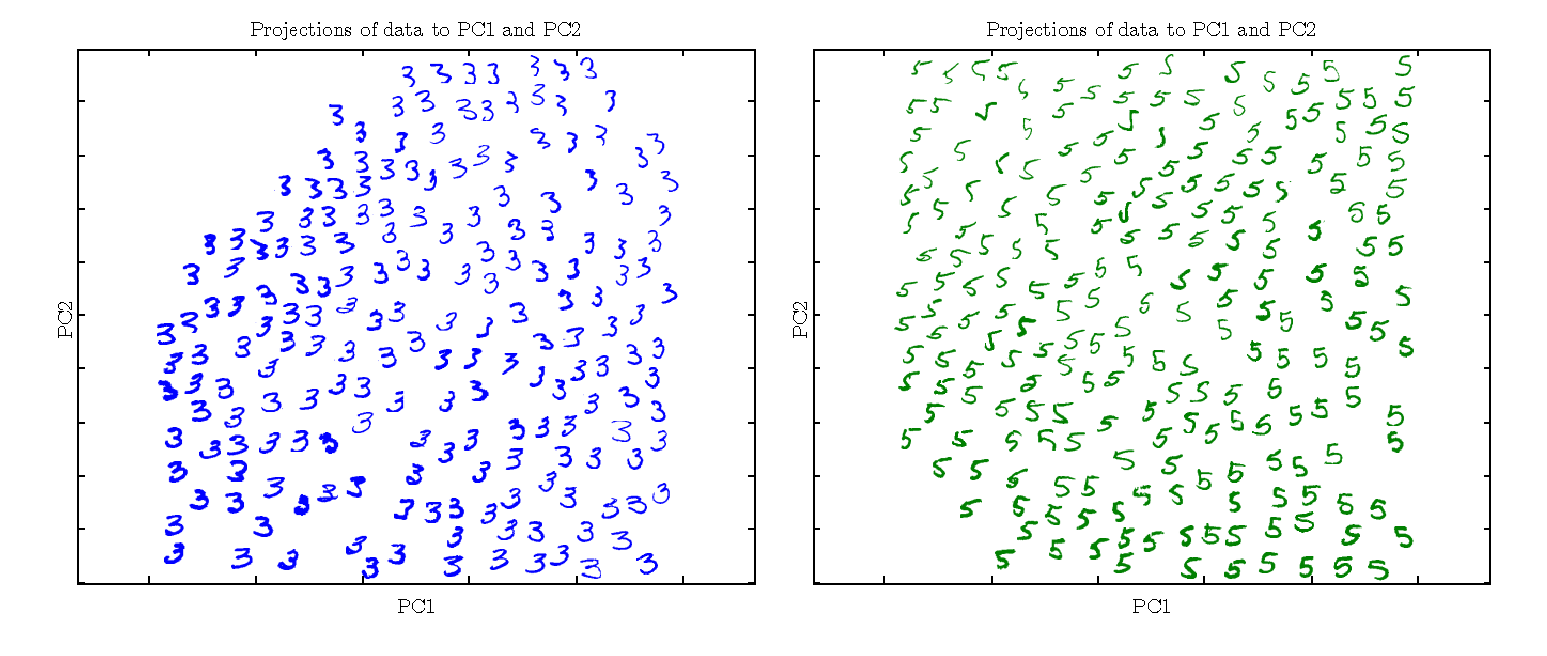
\includegraphics[width=1\linewidth]{code/pca_digit_cluster_z}
\caption{}
\label{fig:pca_cluster_zoom}
\end{figure}


\section{Gaussian Mixture Model (GMM)}

As asked in the assignment we have clustered our data by the Gaussian Mixture Model and used cross-validation to determine the how many clusters produces the best results. \\

Since our data set (again) is too big such that we are unable to run this in a decent time, we have had to take some measures to bring the runtime down. As such we have decided to use the 40 first principal components from a PCA over the digits, instead of the 272 original attributes. We have also cut the observation size down from 60.000 to 10.000, and even with all this it is still incredibly compute heavy and takes ages to run. \\

The result using different amount of clusters ($K$) is shown below.

\begin{figure}[H]
\centering
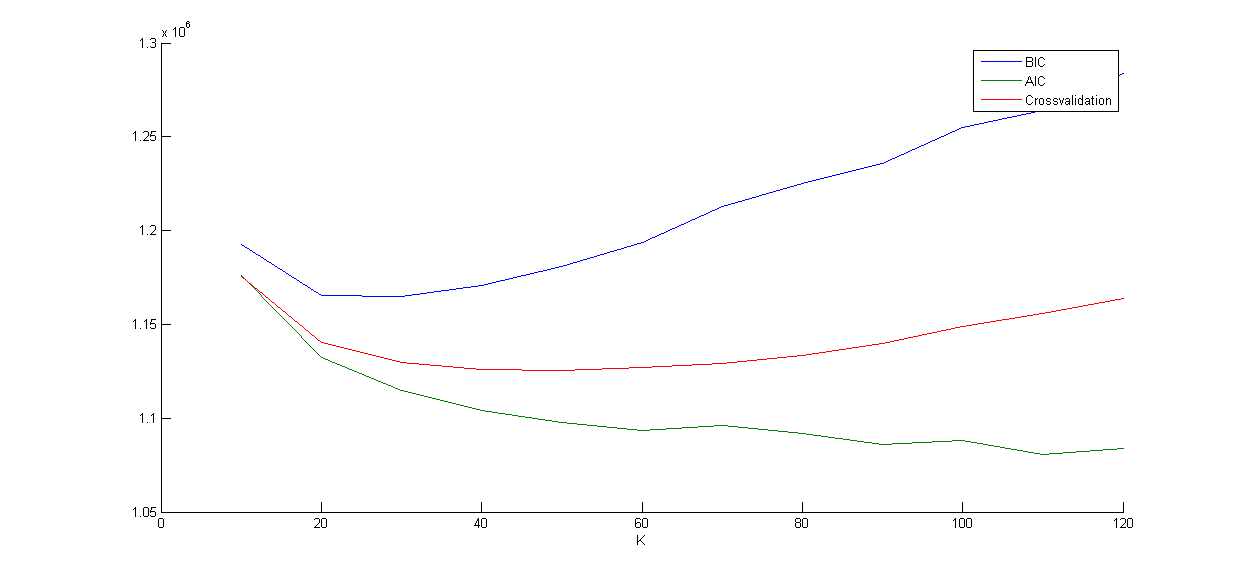
\includegraphics[width=1\linewidth]{code/pca_gmm10-120_cv}
\caption{The y-axis is the negative logarithm-likelihood for each amount of clusters $K$. Besides cross-validation, AIC and BIC are also plotted on the graph. One can see that the maximum likelihood is around K=50 for CV.}
\label{fig:pca_gmm10-120_cv}
\end{figure}


From this we can conclude that when using this clustering method with cross-validation on all 10 of our digits, we need to use 50 clusters to get the best result.


\section{Hierarchical clustering}

Every time we try to run the functions to do any hierarchical clustering it errors out because of too high recursion or some indexing errors. It seems that it is simply too much data for the function(s) to handle, and because of that we have not been able to get any result using this clustering technique.


